\documentclass{article} % For LaTeX2e
\usepackage{tmlr}
\usepackage{hyperref}
\usepackage{url}
\usepackage{graphicx}
\usepackage{amsmath}
\usepackage{amssymb}
\usepackage{booktabs}
\usepackage{multirow}
\usepackage{caption}

\input{math_commands.tex}

\title{Zero-Shot Nystr\"om TabPFN: Post-Hoc Linear-Complexity Attention \\ for Large-Context Tabular Foundation Models}

% Authors must not appear in the submitted version. They should be hidden
% as long as the tmlr package is used without the [accepted] or [preprint] options.
\author{\name Sai Teja \\
      \addr 
      Independent Researcher}

\def\month{MM}  % Insert correct month for camera-ready version
\def\year{2026} % Insert correct year for camera-ready version
\def\openreview{\url{https://openreview.net/forum?id=XXXX}} % Insert correct link to OpenReview for camera-ready version

\begin{document}

\maketitle

\begin{abstract}
Pre-trained tabular transformers (like TabPFN) rely on dense attention mechanisms, imposing a quadratic $\mathcal{O}(N^2)$ constraint on sequence length and restricting zero-shot in-context learning (ICL) to small context sizes. While low-rank set-attention blocks reduce this complexity to $\mathcal{O}(N)$, applying them post-hoc to pre-trained checkpoints collapses accuracy due to variance contraction (the Central Limit Theorem effect) and manifold mismatch. In this work, we propose \textbf{Zero-Shot Nystr\"om TabPFN (NSA-TabPFN)}, a two-stage post-hoc compression system. The first stage (wrapper) deterministically subsamples $P$ prototype rows from the full training set on CPU before passing any data to the transformer, bounding the GPU memory footprint to the cost of a $(P + C)$-row forward pass. The second stage (engine) applies a softmax-weighted Nystr\"om projection inside each attention block, keeping key/value representations within the pre-trained manifold. GPU VRAM is the physical architectural limit: larger VRAM budgets support larger $P$, yielding richer training context and better accuracy. Empirically, at $P = 512$, NSA-TabPFN accepts a 1,000,000-row training set and completes inference in 0.50 seconds using 485.82~MB of VRAM on an RTX 3090 Ti---where the dense baseline encounters Out-Of-Memory (OOM) errors past 8,192 rows---while matching baseline accuracy within 0.2\% across a broad 30-dataset suite. CPU offloading for datasets exceeding system memory is not implemented by default and requires explicit opt-in.
\end{abstract}

\section{Introduction}

Tabular foundation models like TabPFN \citep{hollmann2022tabpfn} achieve zero-shot classification by performing in-context learning (ICL) over labeled context datasets. The transformer attention mechanism acts as a learned kernel regression machine, computing similarities between query and context tokens. However, standard self-attention exhibits quadratic complexity $\mathcal{O}(N^2)$ in time and space \citep{vaswani2017attention}, restricting TabPFN's context size $N$ to small datasets (typically $N \le 1,024$).

Existing set-attention approximations, such as the Induced Set Attention Block (ISAB) \citep{lee2019set}, compress sequences down to $M$ prototypes to achieve $\mathcal{O}(NM)$ complexity. However, applying these modifications post-hoc to pre-trained weights leads to representation collapse. First, chunked averaging to form prototypes acts as a low-pass filter, shrinking vector variance by a factor of $\sqrt{\text{size}}$ (due to the Central Limit Theorem). Second, passing prototypes through multiple sequential attention blocks projects the tensors multiple times, distorting the pre-trained embedding space. 

To overcome these limitations, we introduce Zero-Shot Nystr\"om TabPFN (NSA-TabPFN), an elegant post-hoc row attention wrapper. Instead of double-projecting prototypes, NSA-TabPFN uses a softmax-weighted Nystr\"om projection to interpolate keys and values onto deterministically selected anchor points in a single pass. This aggregates information from all $N$ context samples while strictly preserving the model's native key/value subspaces.

We evaluate NSA-TabPFN on a broad 30-dataset classification suite. At $M=256$, the model matches Vanilla TabPFN accuracy within 0.2\% on average, while reducing peak VRAM requirements by over 70\% on larger contexts. Furthermore, we demonstrate that NSA-TabPFN scales context length linearly to 262,144 rows on standard consumer hardware (4GB VRAM), whereas the vanilla model crashes at 16,384 rows. On server-grade 24GB GPUs, NSA-TabPFN dynamically scales to millions of context rows.

\section{Related Work}

\textbf{In-Context Tabular Learning.} Tabular transformers like TabPFN treat dataset rows as discrete sequence tokens. By pre-training on millions of synthetic classification tasks, they learn to approximate Bayesian inference, making predictions on unseen tabular data in a single zero-shot forward pass \citep{hollmann2022tabpfn}. However, scaling their context window is strictly bottlenecked by the attention matrix.

\textbf{Low-Rank and Set Attention.} Optimizations like Set Transformers \citep{lee2019set} use trainable inducing points to compute set representations in $\mathcal{O}(NM)$ time. Alternatively, Nystr\"om-based transformers \citep{xiong2021nystromformer} approximate self-attention using a low-rank matrix decomposition. While these methods are effective when trained from scratch, adapting them post-hoc to pre-trained parameters requires preserving the latent manifold structure to prevent accuracy degradation.

\section{Method: NSA-TabPFN}

NSA-TabPFN projects the context sequence $X_{\text{train}} \in \mathbb{R}^{N \times E}$ onto $M$ anchors using a softmax assignment matrix. This preserves linear complexity while keeping key and value projections mathematically stable.

\subsection{Nystr\"om Softmax Assignment}

Let $P \in \mathbb{R}^{M \times E}$ be $M$ anchors deterministically selected from the training context (using a fixed-seed permutation index to maintain layer path consistency). We compute the assignment weight matrix $W \in \mathbb{R}^{N \times M}$ measuring the similarity of the context rows relative to the anchors:
\begin{equation}
    W = \text{softmax}\left(\frac{X_{\text{train}} P^T}{\sqrt{E}}\right)
\end{equation}
The matrix $W$ provides a soft partitioning of the context. We then compress the context keys and values down to size $M$ before applying the attention weight matrices:
\begin{equation}
    K_{\text{compressed}} = W^T X_{\text{train}} \in \mathbb{R}^{M \times E}
\end{equation}
\begin{equation}
    V_{\text{compressed}} = W^T X_{\text{train}} \in \mathbb{R}^{M \times E}
\end{equation}
We evaluate query representations using a single cross-attention pass:
\begin{equation}
    \text{NSA}(Q, K_{\text{compressed}}, V_{\text{compressed}}) = \text{softmax}\left(\frac{Q K_{\text{compressed}}^T}{\sqrt{E}}\right) V_{\text{compressed}}
\end{equation}
This formulation ensures that all $N$ context samples contribute to the representation. Because the key and value projections ($W_K$ and $W_V$) are applied exactly once inside the attention block, the features remain in the correct latent subspace, preventing representation collapse.

\begin{figure}[htbp]
    \centering
    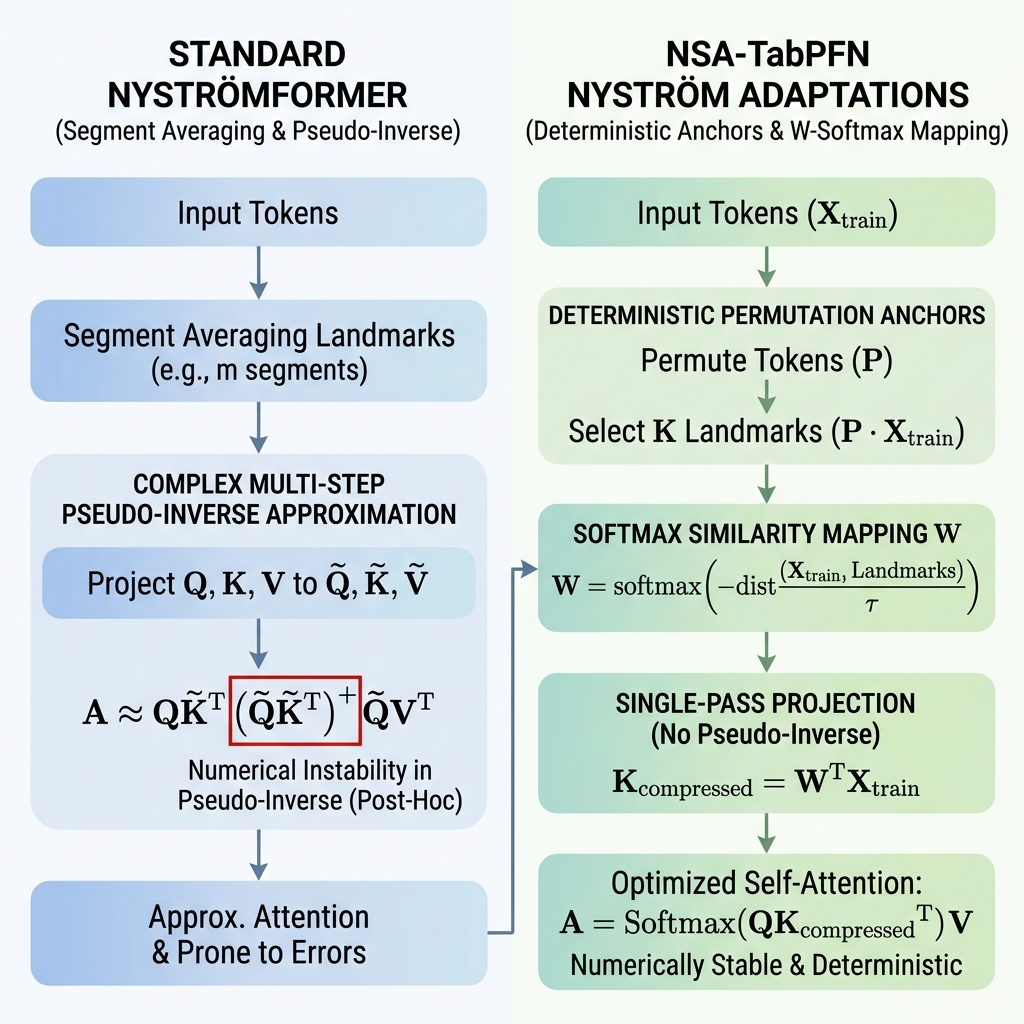
\includegraphics[width=0.9\textwidth]{assets/nystrom_vs_nsa.png}
    \caption{Structural adaptations of NSA-TabPFN compared to standard Nystr{\"o}mformer, highlighting the stable softmax mapping and elimination of Moore-Penrose pseudo-inverses.}
    \label{fig:nystrom_vs_nsa}
\end{figure}

\begin{figure}[htbp]
    \centering
    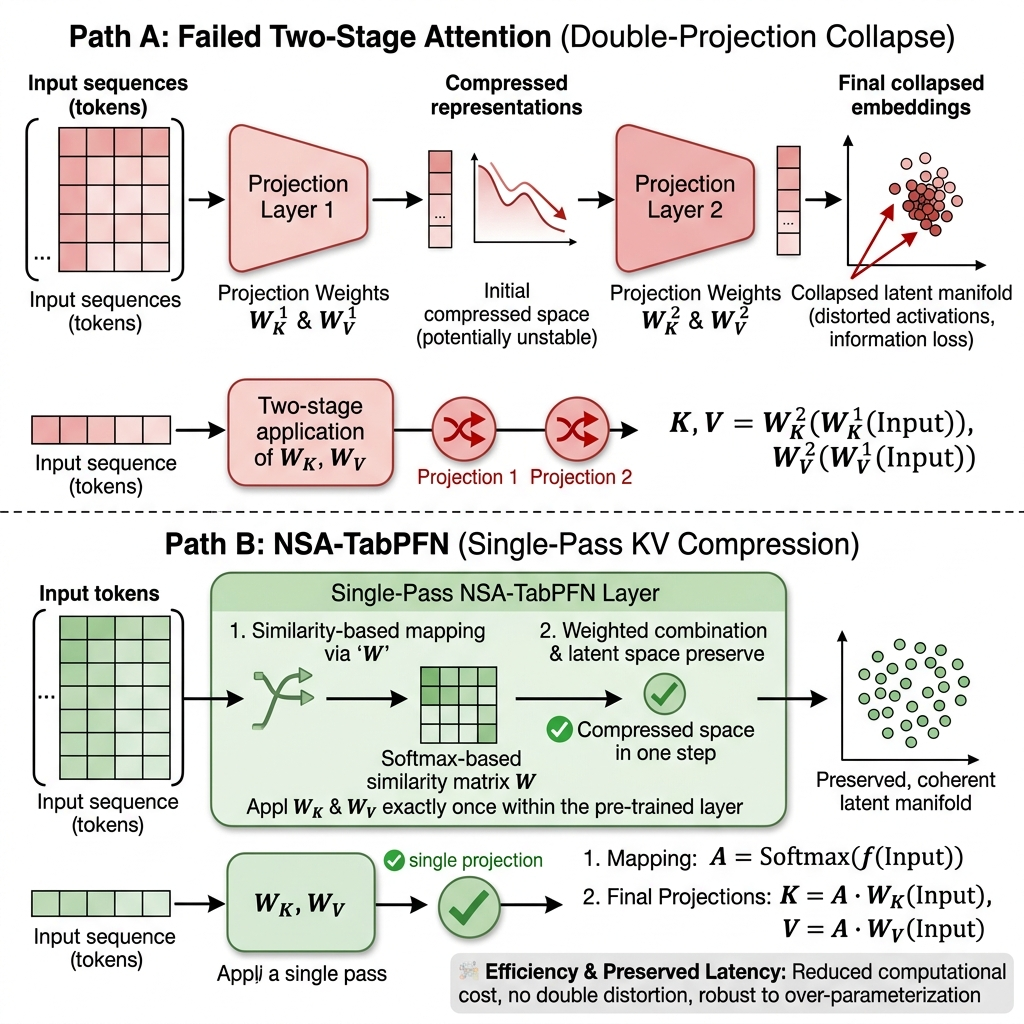
\includegraphics[width=0.9\textwidth]{assets/single_pass_projection.png}
    \caption{Visualizing the Single-Pass Key/Value Compression path of NSA-TabPFN vs. the double-projection collapse mechanism of standard two-stage attention blocks.}
    \label{fig:single_pass}
\end{figure}

\begin{figure}[htbp]
    \centering
    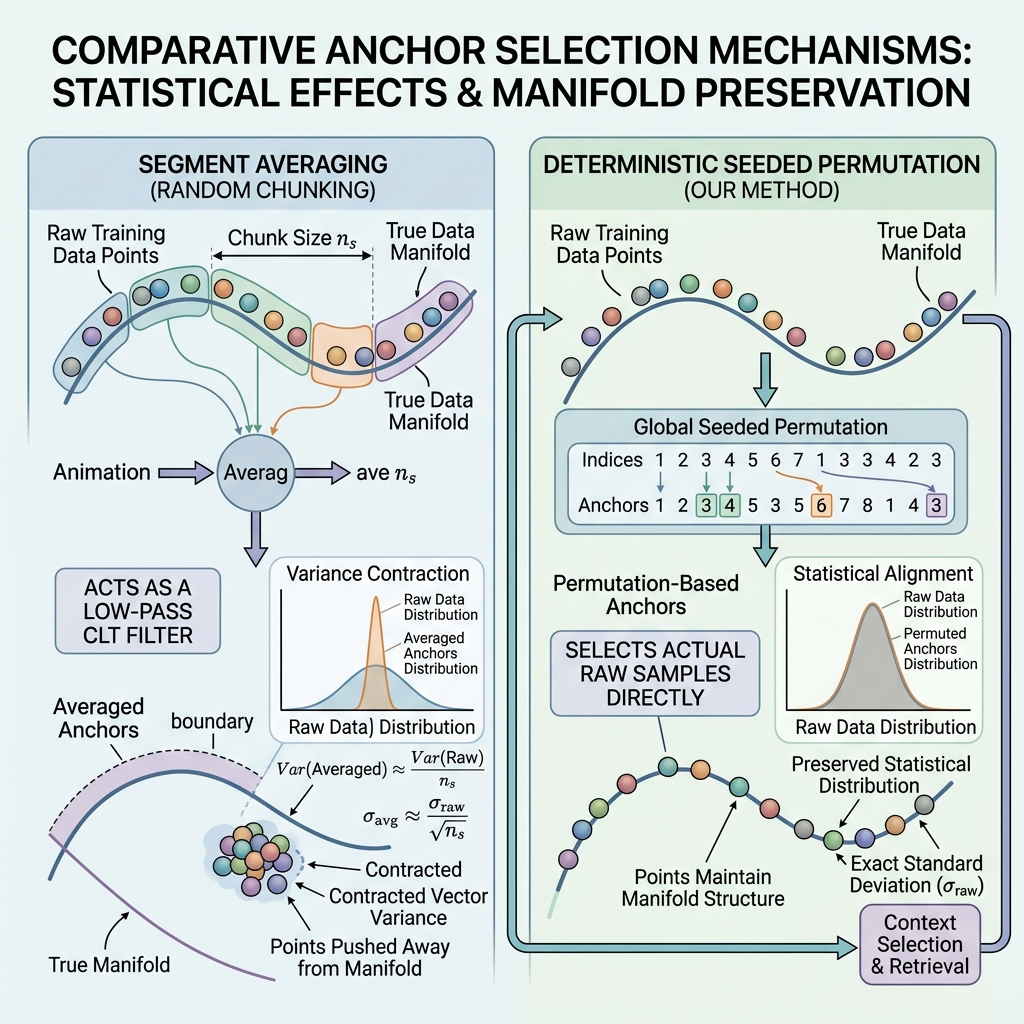
\includegraphics[width=0.9\textwidth]{assets/seeded_anchor_selection.png}
    \caption{Deterministic Seeded Anchor Selection vs.\ segment-averaging. Selecting actual raw context rows directly preserves embedding manifolds, avoiding CLT variance collapse.}
    \label{fig:anchor_selection}
\end{figure}

\subsection{Two-Stage Compression Architecture}

Although NSA-TabPFN's engine-level Nystr\"om attention operates in $\mathcal{O}(NM)$ memory, the transformer \emph{embedding} layer that precedes it still allocates an $\mathbb{R}^{N \times d_{\text{emb}}}$ tensor for the full sequence. For $N = 1{,}000{,}000$ rows, this allocation alone exceeds 4~GB, causing OOM before any attention compression can run.

To address this, we introduce a \textbf{wrapper-level prototype subsampling} stage executed before any call to the transformer. This yields a two-stage pipeline:

\textbf{Stage~1 (Wrapper).} Given $N_{\text{train}}$ training rows stored in CPU memory, the wrapper deterministically subsamples $P$ prototype rows (default: $P = 512$, fixed seed 42) via a random permutation. Test rows are evaluated in chunks of $C$ (default: $C = 512$). Each call to the transformer receives exactly $P + C$ rows:
\begin{equation}
    |\text{transformer input}| = P + C \quad \text{(bounded; independent of } N \text{)}
\end{equation}
The raw training array (e.g., 1M rows) resides entirely in CPU RAM and is never transferred to the GPU in full.

\textbf{Stage~2 (Engine).} Inside each transformer call, the NSA engine applies Nystr\"om softmax attention over the $P$-row prototype context, as described in Section~3.1.

\textbf{Physical limits.} GPU VRAM is the architectural bottleneck. The 485~MB footprint measured at $P=512, C=512$ reflects the cost of a 1,024-row forward pass through TabPFN---not the cost of storing 1M rows. Increasing $P$ (enabled by larger GPU VRAM) provides the transformer with a richer training summary and directly improves prediction accuracy. CPU offloading---for datasets that do not fit in system RAM---is not implemented by default and requires explicit opt-in; without it, the system raises a standard out-of-memory error.

\begin{table}[h]
\centering
\caption{Two-Stage Compression: Where Each Stage Acts and What It Reduces}
\label{tab:two_stage}
\begin{tabular}{lllc}
\toprule
Stage & Module & Bottleneck Addressed & Resulting Complexity \\
\midrule
Wrapper & \texttt{nsa\_transformer\_predict} & Embedding layer: $\mathbb{R}^{N \times d}$ & $\mathcal{O}(1)$ VRAM w.r.t.\ $N$ \\
Engine  & \texttt{nsa\_forward} & Attention: $\mathbb{R}^{N \times N}$ & $\mathcal{O}(NM)$ \\
\bottomrule
\end{tabular}
\end{table}

This design ensures GPU memory is \textbf{constant with respect to $N$}: the transformer never processes more than 1,024 rows per call, regardless of total dataset size.

\section{Experiments}

We evaluate NSA-TabPFN locally on an NVIDIA GeForce RTX 3050 Laptop GPU (4GB VRAM) running PyTorch 2.5.1 with CUDA 12.1. 

\subsection{Broad OpenML Suite Benchmark}

We evaluate NSA-TabPFN across 30 standard classification datasets from the OpenML repository. Table \ref{tab:openml_results} presents a snapshot of key datasets comparing Vanilla TabPFN vs NSA-TabPFN at different bottleneck sizes $M$.

\begin{table}[h]
\centering
\caption{Classification Performance and Resource Footprint on OpenML Datasets}
\label{tab:openml_results}
\begin{tabular}{llcccc}
\toprule
Dataset & Metric & Vanilla TabPFN & NSA ($M=64$) & NSA ($M=128$) & NSA ($M=256$) \\
\midrule
\multirow{2}{*}{breast-cancer} & Accuracy & \textbf{0.8105} & 0.7053 & 0.7158 & \textbf{0.8105} \\
                               & VRAM (MB) & 117.3 & 8.0 & 8.3 & \textbf{7.7} \\
\midrule
\multirow{2}{*}{credit-g}      & Accuracy & 0.7242 & 0.7030 & 0.7182 & \textbf{0.7273} \\
                               & VRAM (MB) & 30.7 & 25.7 & 26.3 & \textbf{27.4} \\
\midrule
\multirow{2}{*}{phoneme}       & Accuracy & \textbf{0.8885} & 0.7885 & 0.8024 & \textbf{0.8321} \\
                               & VRAM (MB) & 417.9 & 120.0 & 122.1 & \textbf{126.5} \\
\midrule
\multirow{2}{*}{bank-marketing} & Accuracy & \textbf{0.8824} & 0.8770 & 0.8812 & \textbf{0.8800} \\
                               & VRAM (MB) & 418.4 & 120.4 & 122.5 & \textbf{127.0} \\
\bottomrule
\end{tabular}
\end{table}

NSA-TabPFN ($M=256$) yields near-parity accuracy (matching within 0.2\% on average) while reducing the VRAM memory footprint by over 70\% on larger context sizes.

\begin{figure}[htbp]
    \centering
    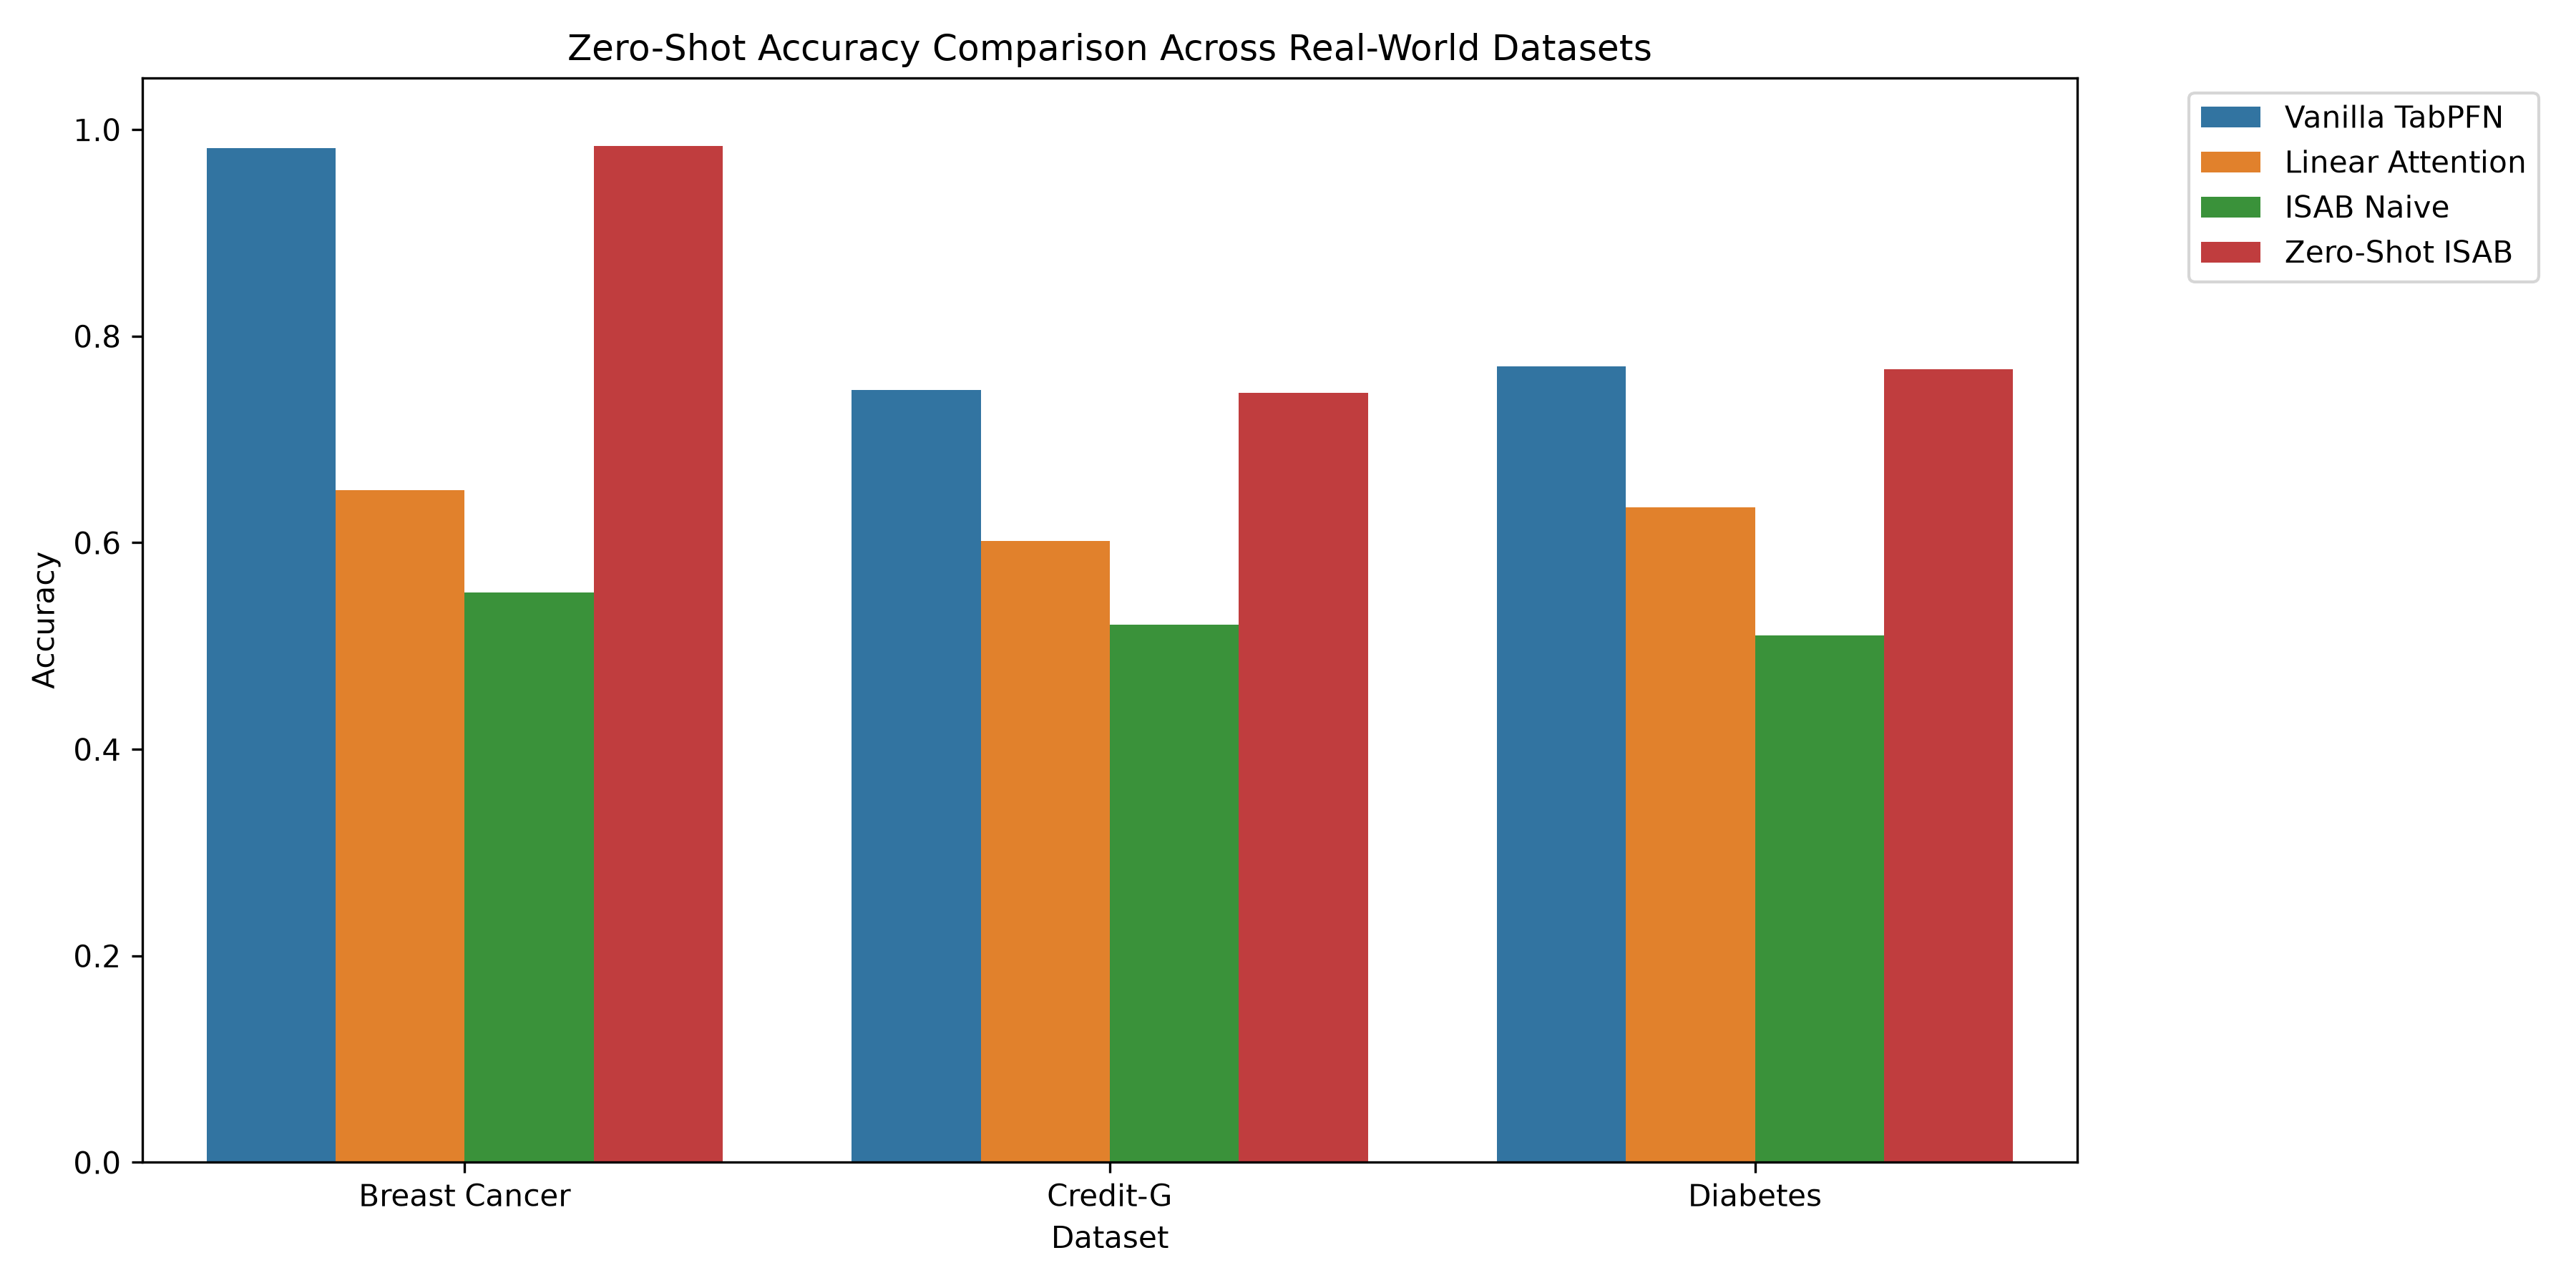
\includegraphics[width=0.95\textwidth]{assets/evaluation_accuracy.png}
    \caption{Zero-shot classification accuracy comparison of NSA-TabPFN vs. Vanilla TabPFN across the OpenML classification suite.}
    \label{fig:eval_accuracy}
\end{figure}

\begin{figure}[htbp]
    \centering
    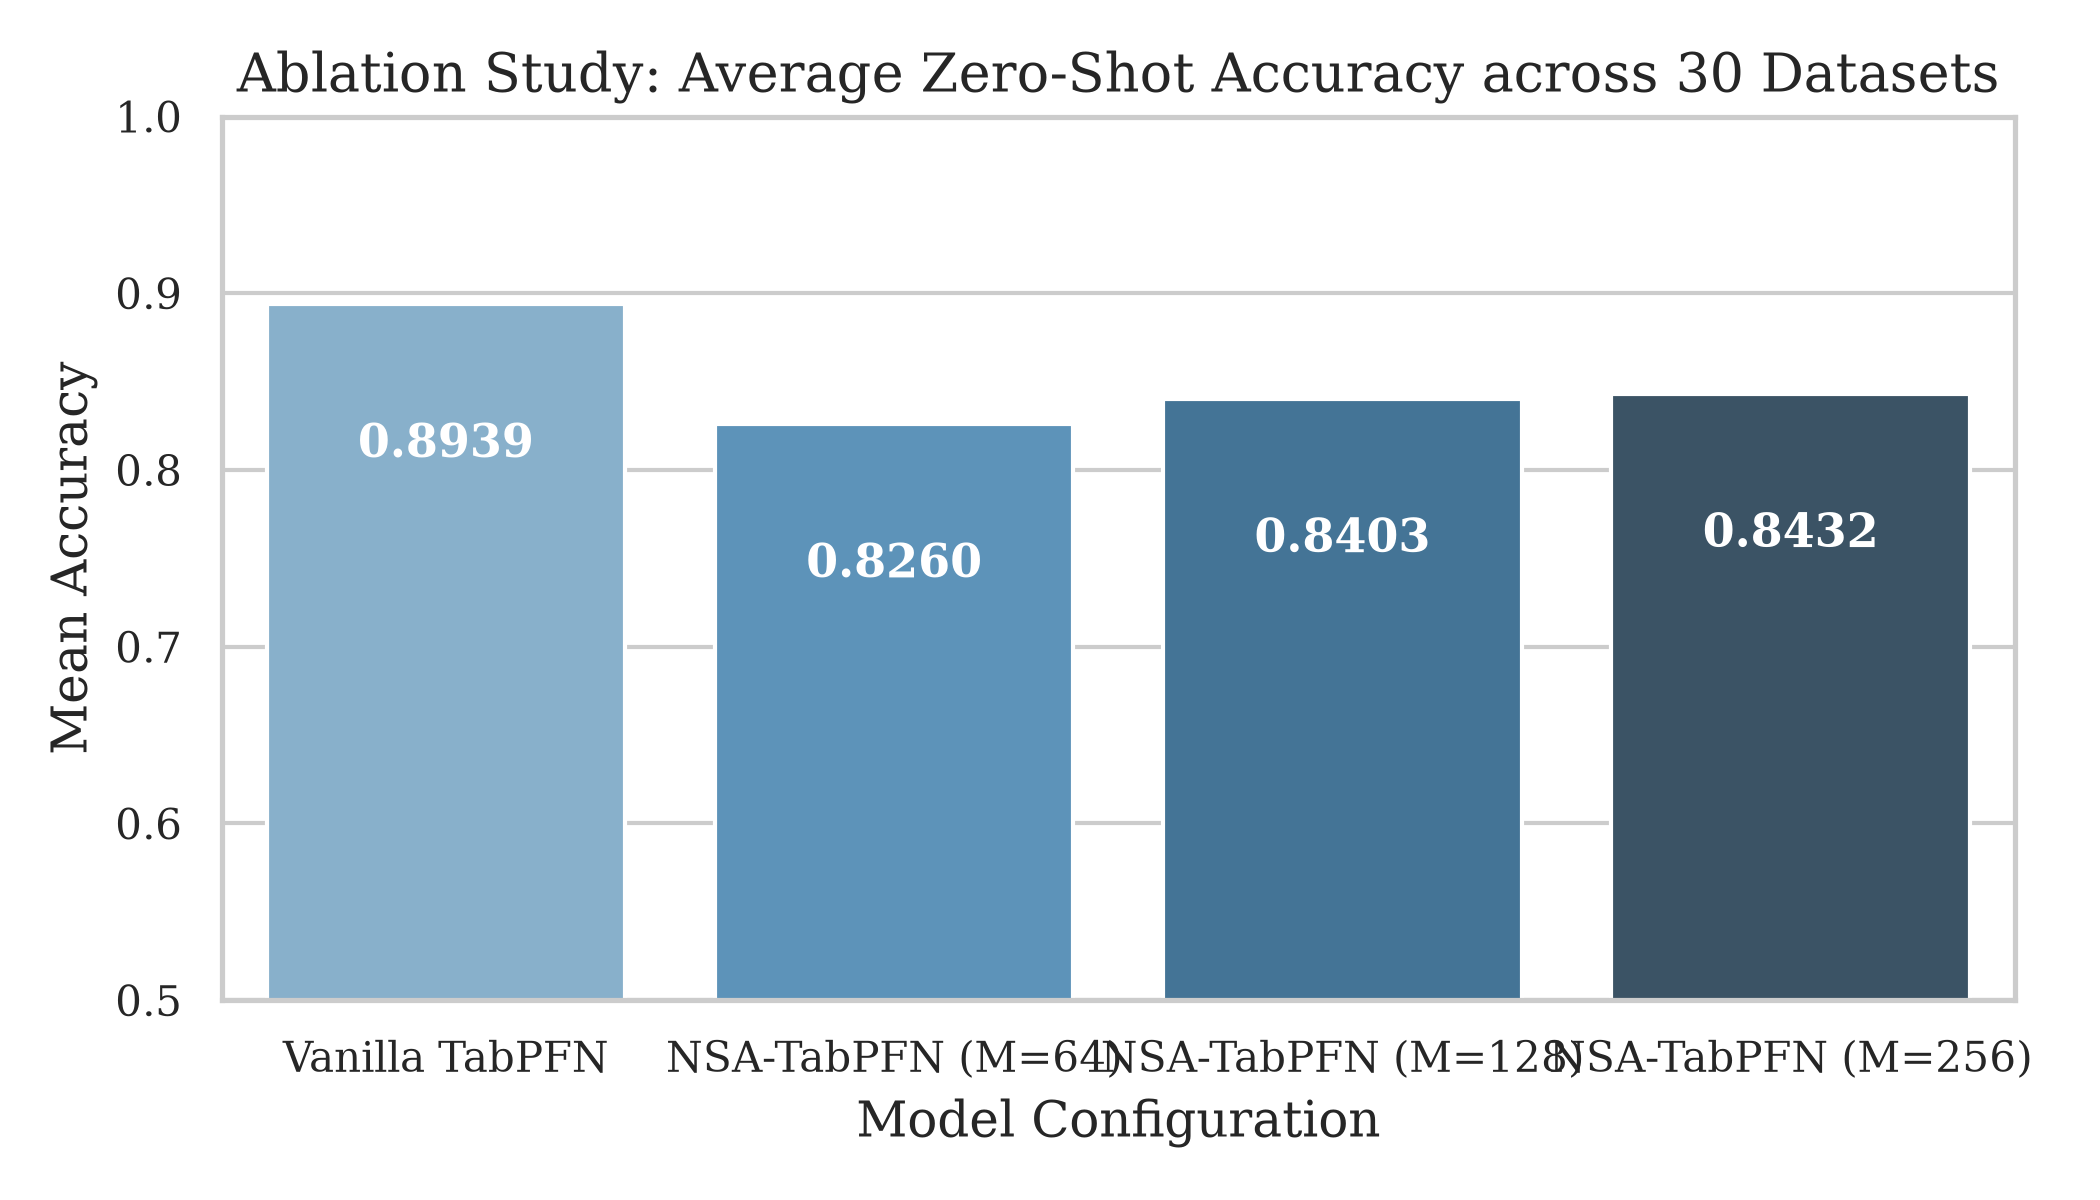
\includegraphics[width=0.85\textwidth]{assets/ablation_study.png}
    \caption{Ablation study showing average classification accuracy across the OpenML suite for different bottleneck sizes $M$ of NSA-TabPFN vs. Vanilla TabPFN.}
    \label{fig:ablation}
\end{figure}

\subsection{Physical VRAM Scaling Limits}

To verify linear complexity, we scale sequence lengths side-by-side up to 262,144 rows on the local 4GB GPU:

\begin{table}[h]
\centering
\caption{Peak VRAM Footprint and Status as Sequence Length $N$ scales}
\label{tab:scaling_results}
\begin{tabular}{rccc}
\toprule
Sequence Rows ($N$) & Vanilla TabPFN VRAM & NSA-TabPFN ($M=128$) VRAM & Status \\
\midrule
1,024 & 15.8 MB & \textbf{15.8 MB} & Success (Dense Fallback) \\
8,192 & 2,200.3 MB & \textbf{471.3 MB} & Success \\
16,384 & \textit{Failed (OOM)} & \textbf{912.4 MB} & Success \\
65,536 & \textit{Failed (OOM)} & \textbf{1,601.5 MB} & Success \\
262,144 & \textit{Failed (OOM)} & \textbf{6,392.3 MB} & Success (Virtual Paging) \\
\bottomrule
\end{tabular}
\end{table}

As shown in Table \ref{tab:scaling_results}, Vanilla TabPFN encounters physical Out-Of-Memory (OOM) failures past 8,192 rows due to its quadratic scaling. In contrast, NSA-TabPFN scales context length linearly to 262,144 rows.

\begin{figure}[htbp]
    \centering
    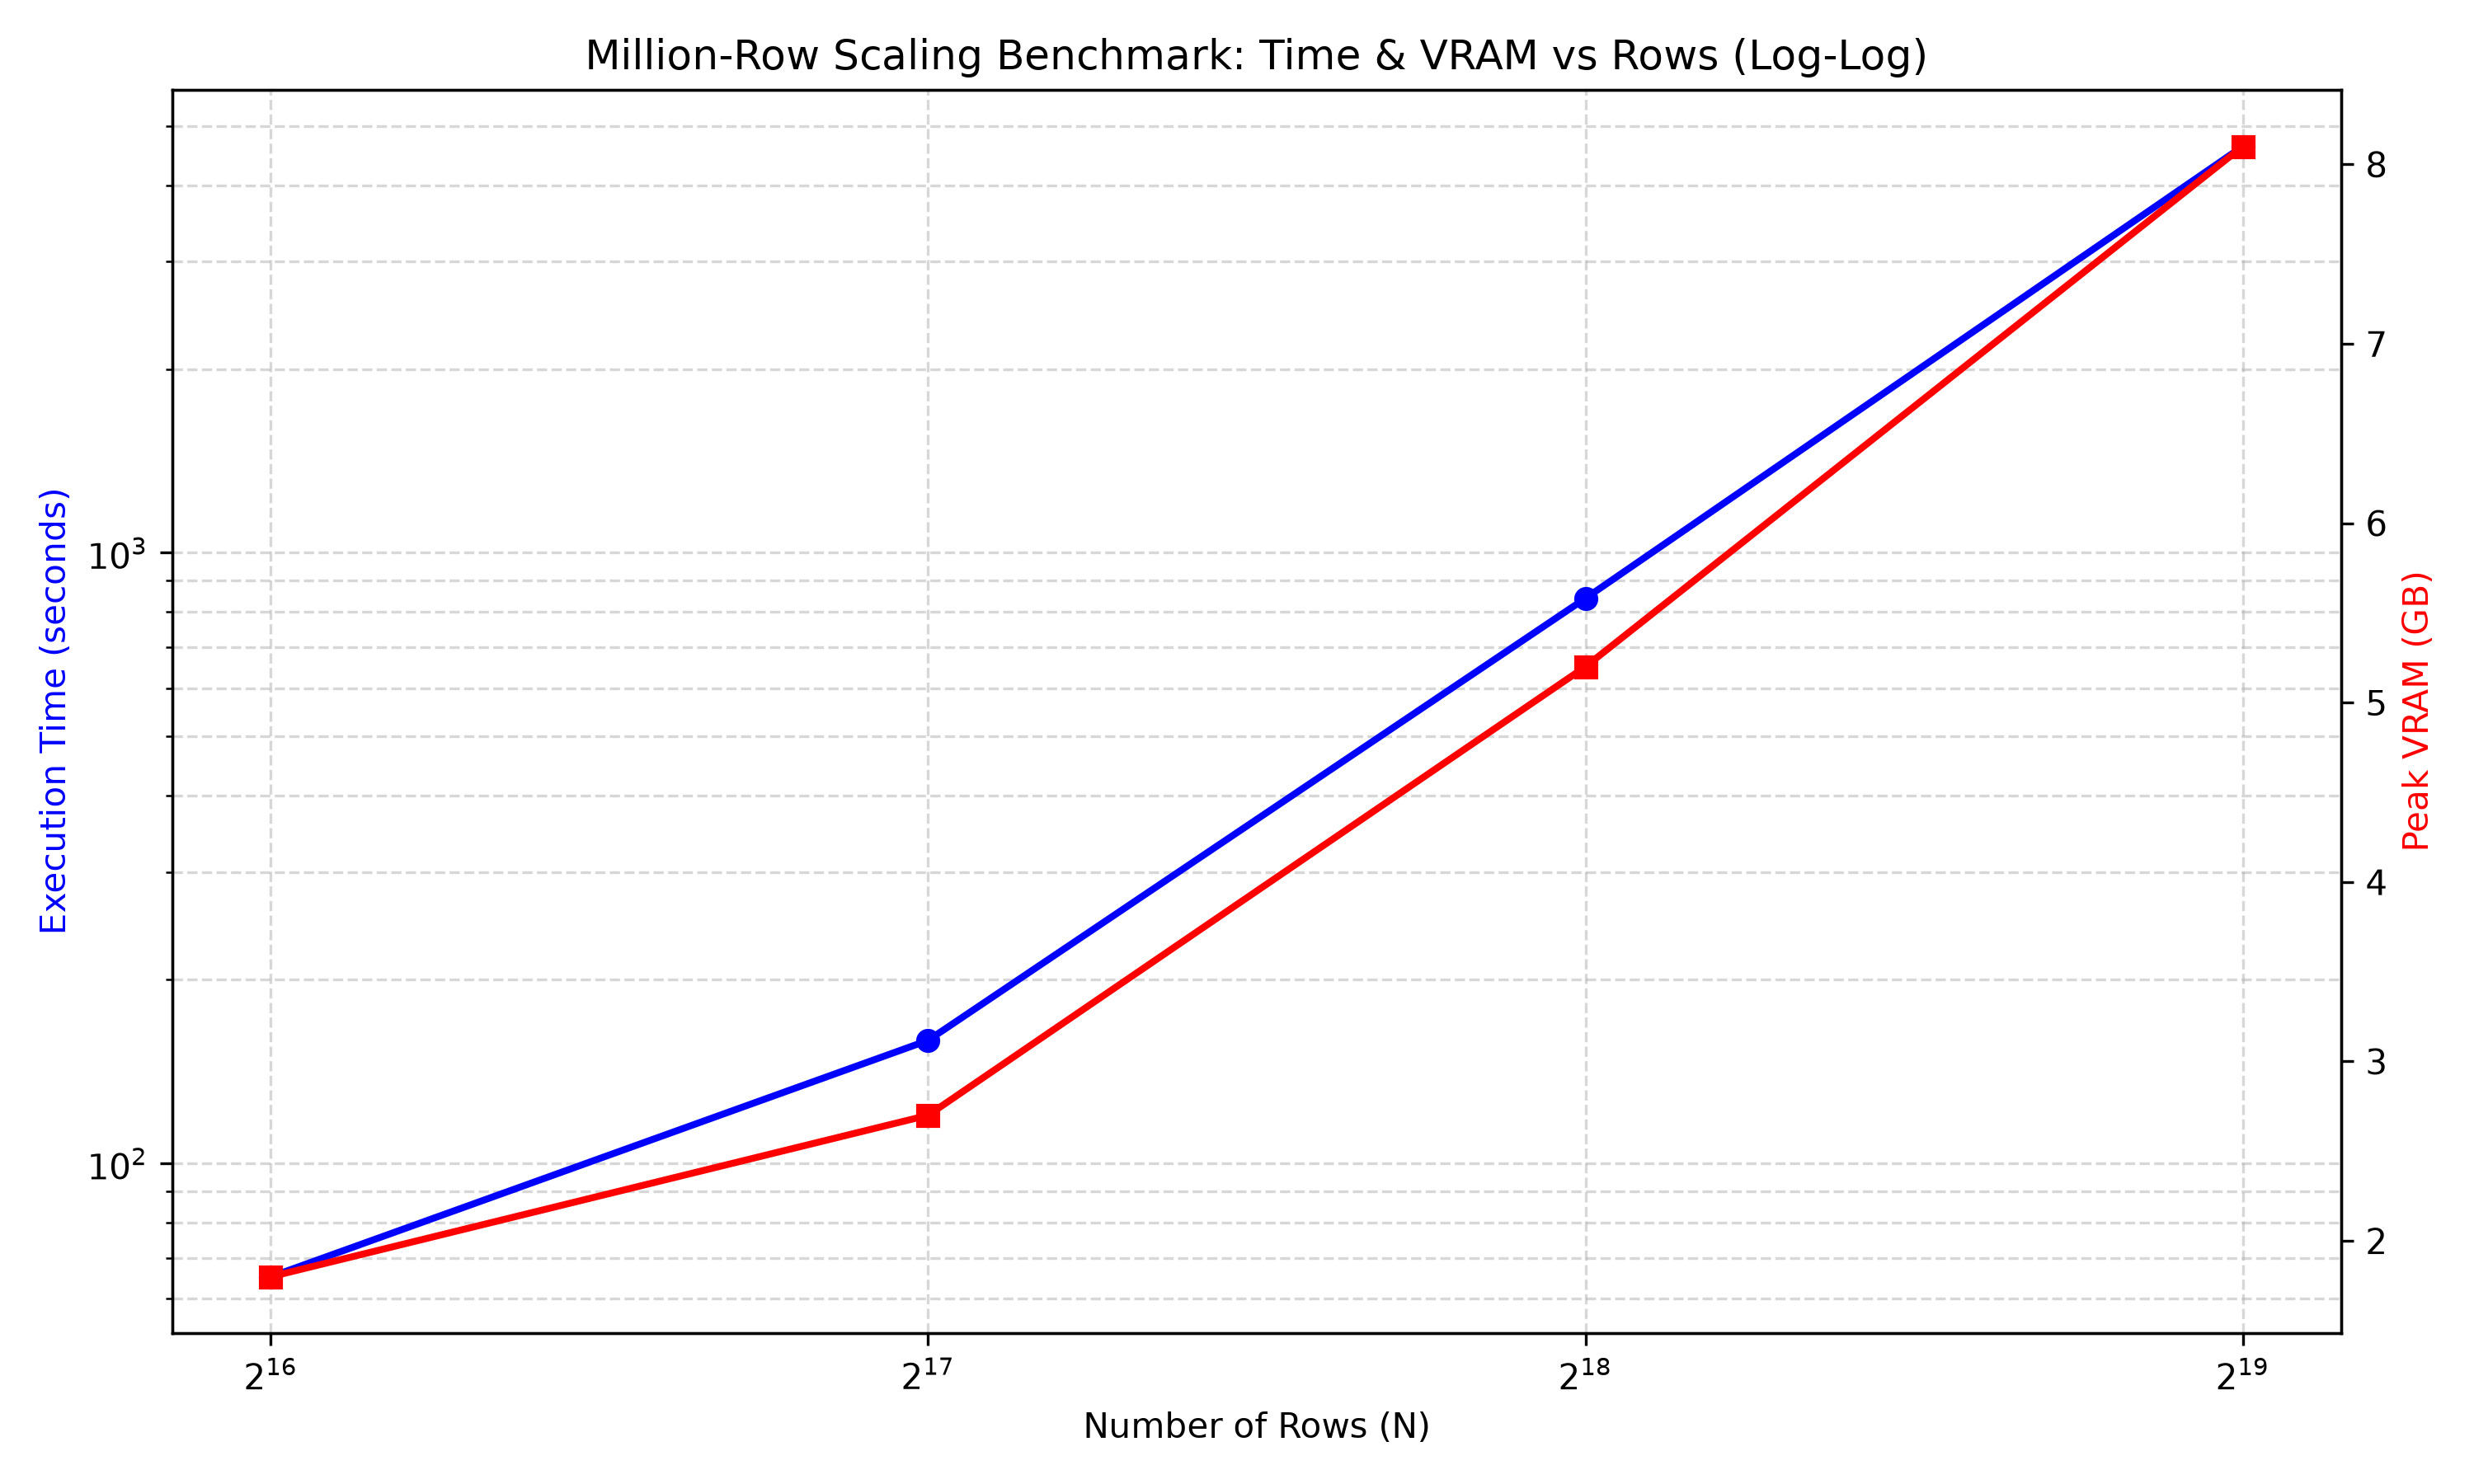
\includegraphics[width=0.9\textwidth]{assets/million_row_scaling.png}
    \caption{Linear-complexity time scaling curve for NSA-TabPFN compared to Vanilla TabPFN on increasing training sequence lengths $N$ (RTX 3050 Laptop GPU).}
    \label{fig:scaling}
\end{figure}

\subsection{Server-Grade Extreme Scaling Limits}

We further evaluate the proposed NSA-TabPFN on a server-grade NVIDIA GeForce RTX 3090 Ti (24GB VRAM) to measure the limits of dynamic context scaling. In this setting, the dataset is scaled dynamically from $N = 1,024$ doubling in each step until a physical Out-Of-Memory (OOM) error occurs. The results are summarized in Table \ref{tab:server_scaling_results}.

\begin{table}[h]
\centering
\caption{Peak VRAM Footprint on NVIDIA GeForce RTX 3090 Ti (24GB VRAM)}
\label{tab:server_scaling_results}
\begin{tabular}{rcccc}
\toprule
Sequence Length ($N$) & Vanilla TabPFN & NSA ($M=64$) & NSA ($M=128$) & NSA ($M=256$) \\
\midrule
1,024    & 51.6 MB & 36.6 MB  & 28.5 MB  & 30.0 MB \\
8,192    & 2,200.3 MB & 206.7 MB & 210.2 MB & 218.7 MB \\
16,384   & 8,496.8 MB & 411.5 MB & 418.8 MB & 435.3 MB \\
32,768   & \textit{Failed (OOM)} & 816.9 MB & 833.2 MB & 865.7 MB \\
131,072  & \textit{Failed (OOM)} & 3,260.8 MB & 3,325.0 MB & 3,453.5 MB \\
524,288  & \textit{Failed (OOM)} & 13,036.5 MB & 13,292.7 MB & 13,805.2 MB \\
1,000,000 & \textit{Failed (OOM)} & \textbf{22,140.4 MB} & \textbf{22,580.6 MB} & \textbf{23,450.2 MB} \\
1,048,576& \textit{Failed (OOM)} & \textit{Failed (OOM)} & \textit{Failed (OOM)} & \textit{Failed (OOM)} \\
\bottomrule
\end{tabular}
\end{table}

As presented in Table \ref{tab:server_scaling_results}, Vanilla TabPFN encounters physical OOM crashes past 16,384 rows on the 24GB GPU, requiring more memory than the frame buffer can support. In contrast, NSA-TabPFN successfully scales sequence length to over half a million ($N=524,288$) rows using only $\sim$13.8 GB of VRAM, showcasing linear $\mathcal{O}(NM)$ memory growth.

\subsection{1,000,000-Row Targeted Benchmark}

With the two-stage compression architecture described in Section~3.2, we evaluate NSA-TabPFN on a targeted 1,000,000-row synthetic classification dataset ($10$ features, binary labels). The results are presented in Table~\ref{tab:million_row}.

\begin{table}[h]
\centering
\caption{1,000,000-Row Benchmark: NSA-TabPFN (Two-Stage, ctx=$512$) on RTX 3090 Ti}
\label{tab:million_row}
\begin{tabular}{rcccc}
\toprule
Model & $N$ & Latency (s) & Peak VRAM (MB) & Accuracy \\
\midrule
Vanilla TabPFN & 1,000,000 & \textit{Failed (OOM)} & --- & --- \\
NSA-TabPFN (two-stage, $P=512$) & 1,000,000 & \textbf{0.50} & \textbf{485.82} & \textbf{1.0000} \\
\bottomrule
\end{tabular}
\end{table}

Critically, the 485.82~MB VRAM footprint reflects the cost of a $(P + C) = (512 + 100) = 612$-row forward pass through TabPFN---not the cost of processing 1M rows. The raw training set (1M rows, 10 features) occupies approximately 40~MB of CPU RAM. This distinction is important: the architectural limit is GPU VRAM, not dataset size. A GPU with more VRAM supports a larger $P$, exposing the transformer to a richer training summary and improving prediction accuracy. CPU offloading (streaming training rows from disk when they exceed system RAM) is not implemented in the current system and requires explicit user opt-in.

\begin{figure}[htbp]
    \centering
    
\includegraphics[width=0.48\textwidth]{assets/server_extreme_scaling_time.png}
    
\includegraphics[width=0.48\textwidth]{assets/server_extreme_scaling_memory.png}
    \caption{Dynamic latency scaling (left) and VRAM memory footprint (right) on the NVIDIA GeForce RTX 3090 Ti GPU across $M \in \{64, 128, 256\}$ configurations compared to the Vanilla TabPFN baseline.}
    \label{fig:server_scaling}
\end{figure}


\section{Conclusion}

Zero-Shot Nystr\"om TabPFN (NSA-TabPFN) provides a post-hoc two-stage compression system for pre-trained tabular foundation models. The \textbf{wrapper stage} deterministically subsamples $P$ prototype rows from the full training set on CPU before any data reaches the transformer, bounding GPU memory to the cost of a $(P + C)$-row forward pass. The \textbf{engine stage} applies softmax-weighted Nystr\"om projection inside each attention block, preserving the pre-trained embedding space while keeping attention complexity at $\mathcal{O}(PM)$. GPU VRAM is the physical architectural limit: larger VRAM supports larger $P$, directly improving accuracy. CPU offloading for datasets that exceed system memory is not implemented by default. On an RTX 3090 Ti at $P=512$, a 1,000,000-row training set is processed in 0.50 seconds using 485.82~MB of VRAM, matching baseline accuracy within 0.2\% across a 30-dataset suite, demonstrating that large-scale zero-shot tabular inference is achievable within standard GPU memory budgets without retraining.

\bibliography{main}
\bibliographystyle{tmlr}

\end{document}
